\begin{figure*}[t]
	\centering
	\begin{tabular}{cccc}
		\hspace{-0.5em}\subfloat[][$\ammd$ vs. $\mm$]{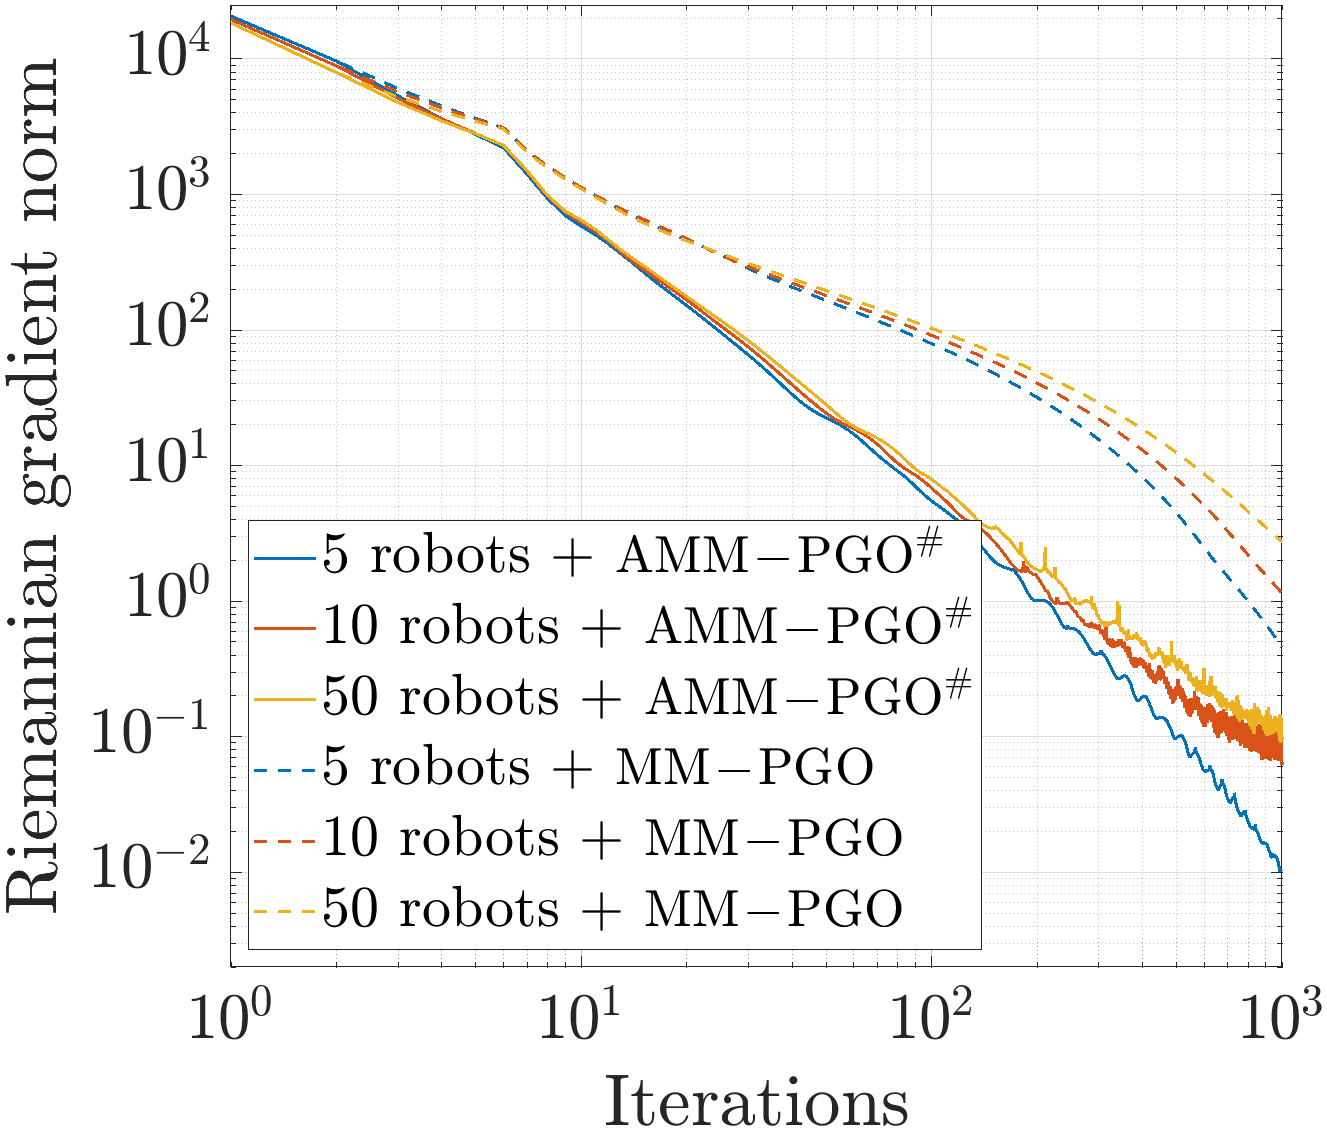
\includegraphics[trim =0mm 0mm 0mm 0mm,width=0.24\textwidth]{figures/cube_tests/rel_huber_g.png}} &
		\hspace{-0.6em}\subfloat[][5 robots]{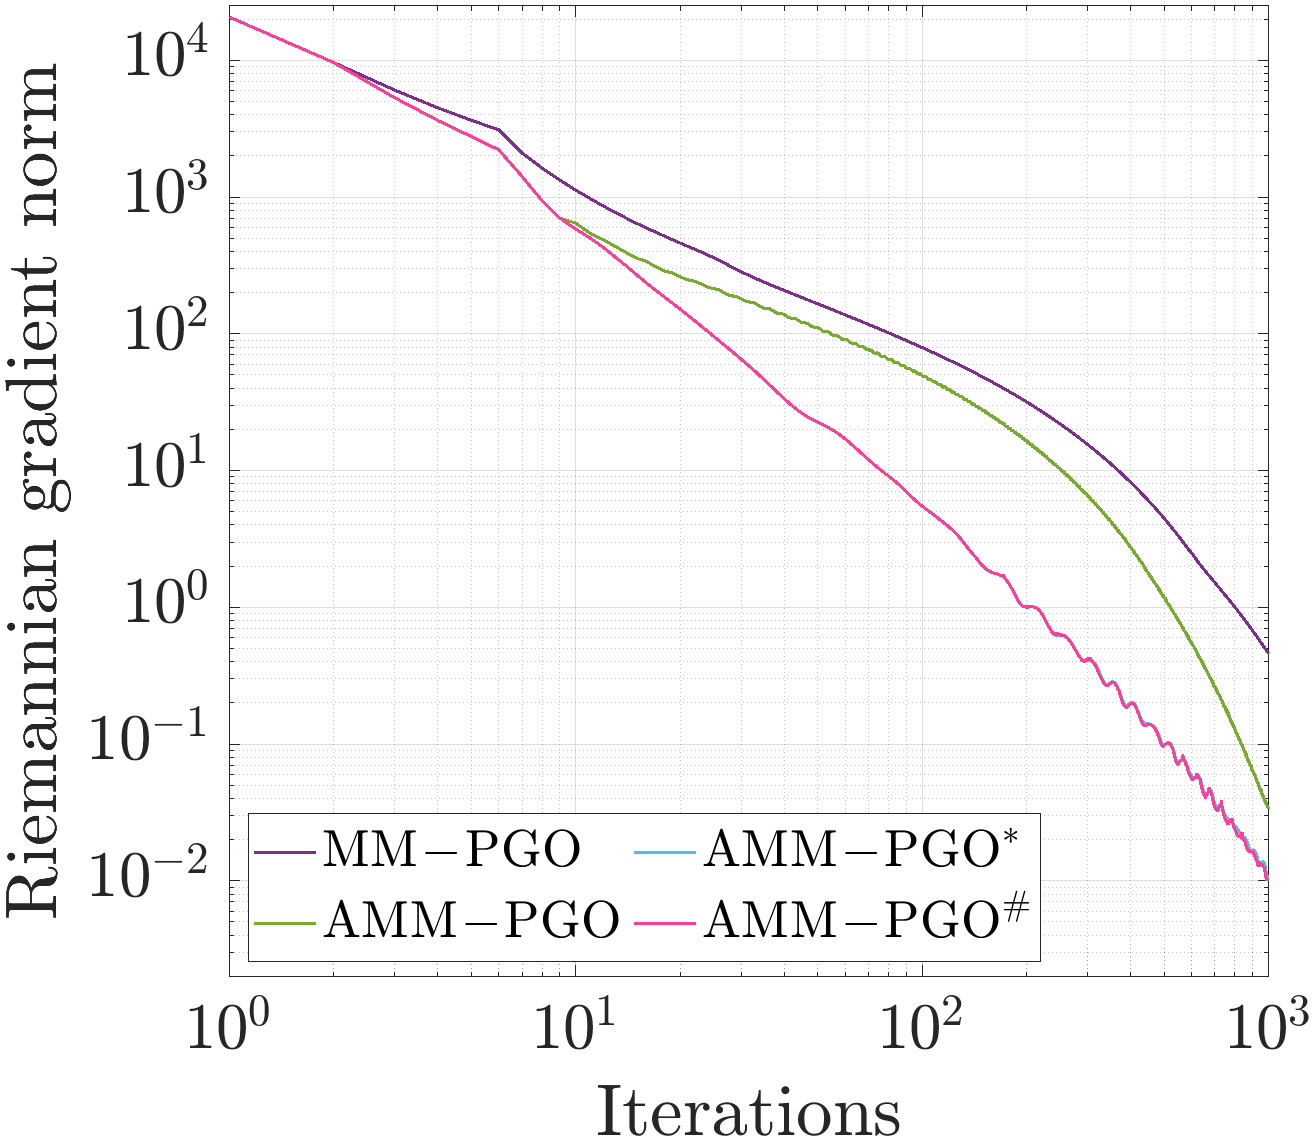
\includegraphics[trim =0mm 0mm 0mm 0mm,width=0.24\textwidth]{figures/cube_tests/rel_huber_g_5.png}} &
		\hspace{-0.6em}\subfloat[][10 robots]{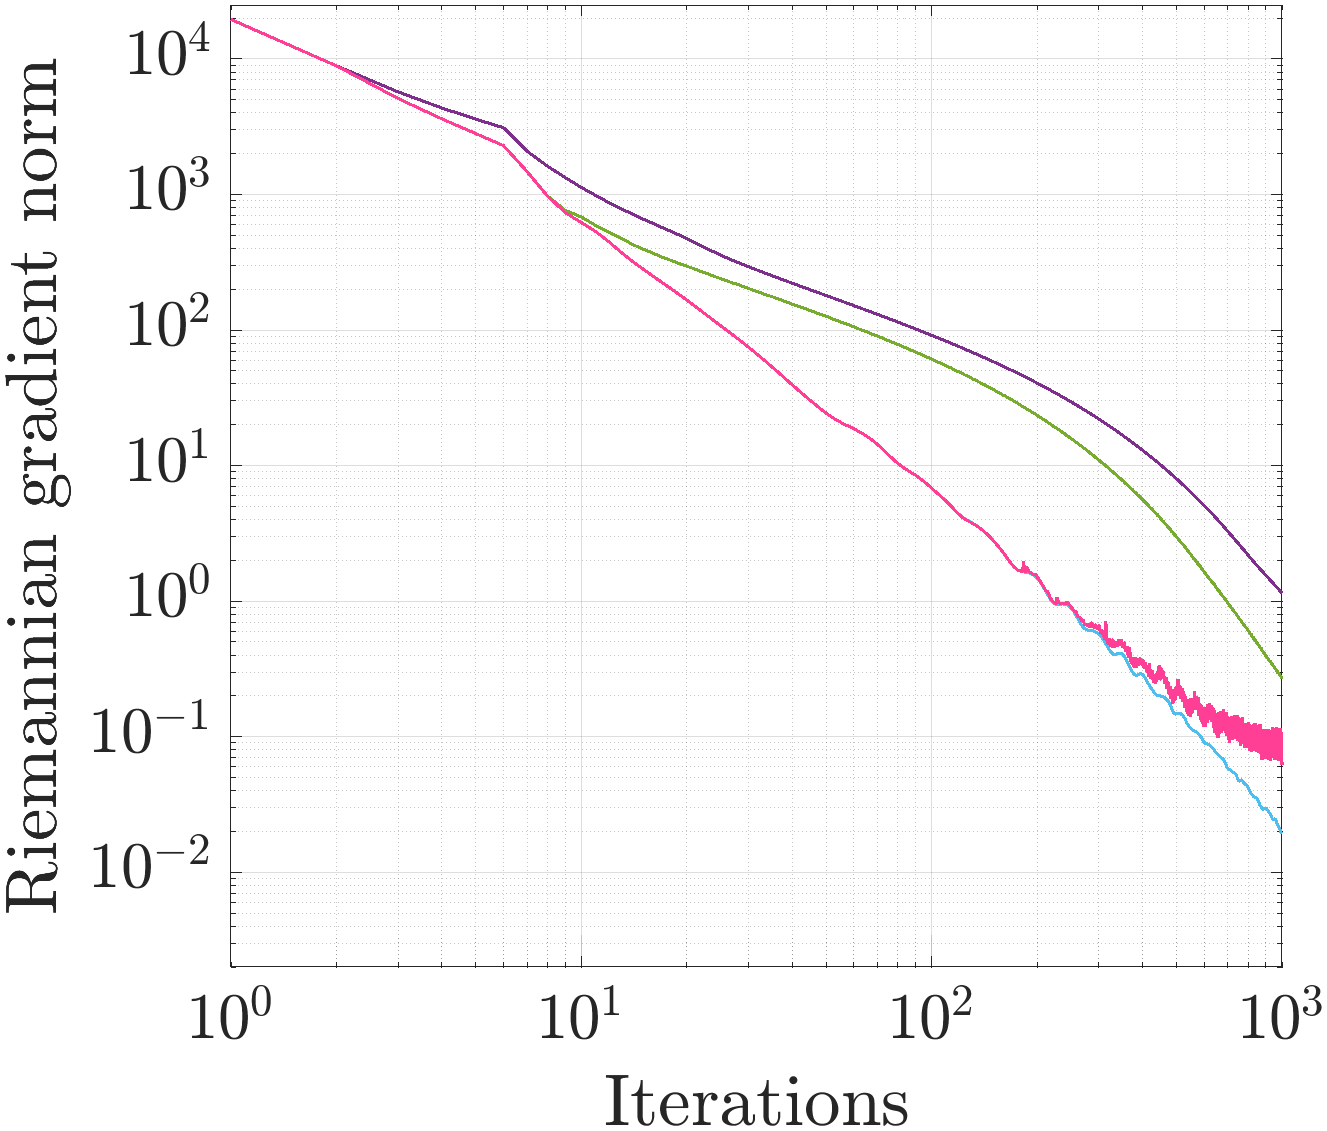
\includegraphics[trim =0mm 0mm 0mm 0mm,width=0.24\textwidth]{figures/cube_tests/rel_huber_g_10.png}}&
		\hspace{-0.6em}\subfloat[][50 robots]{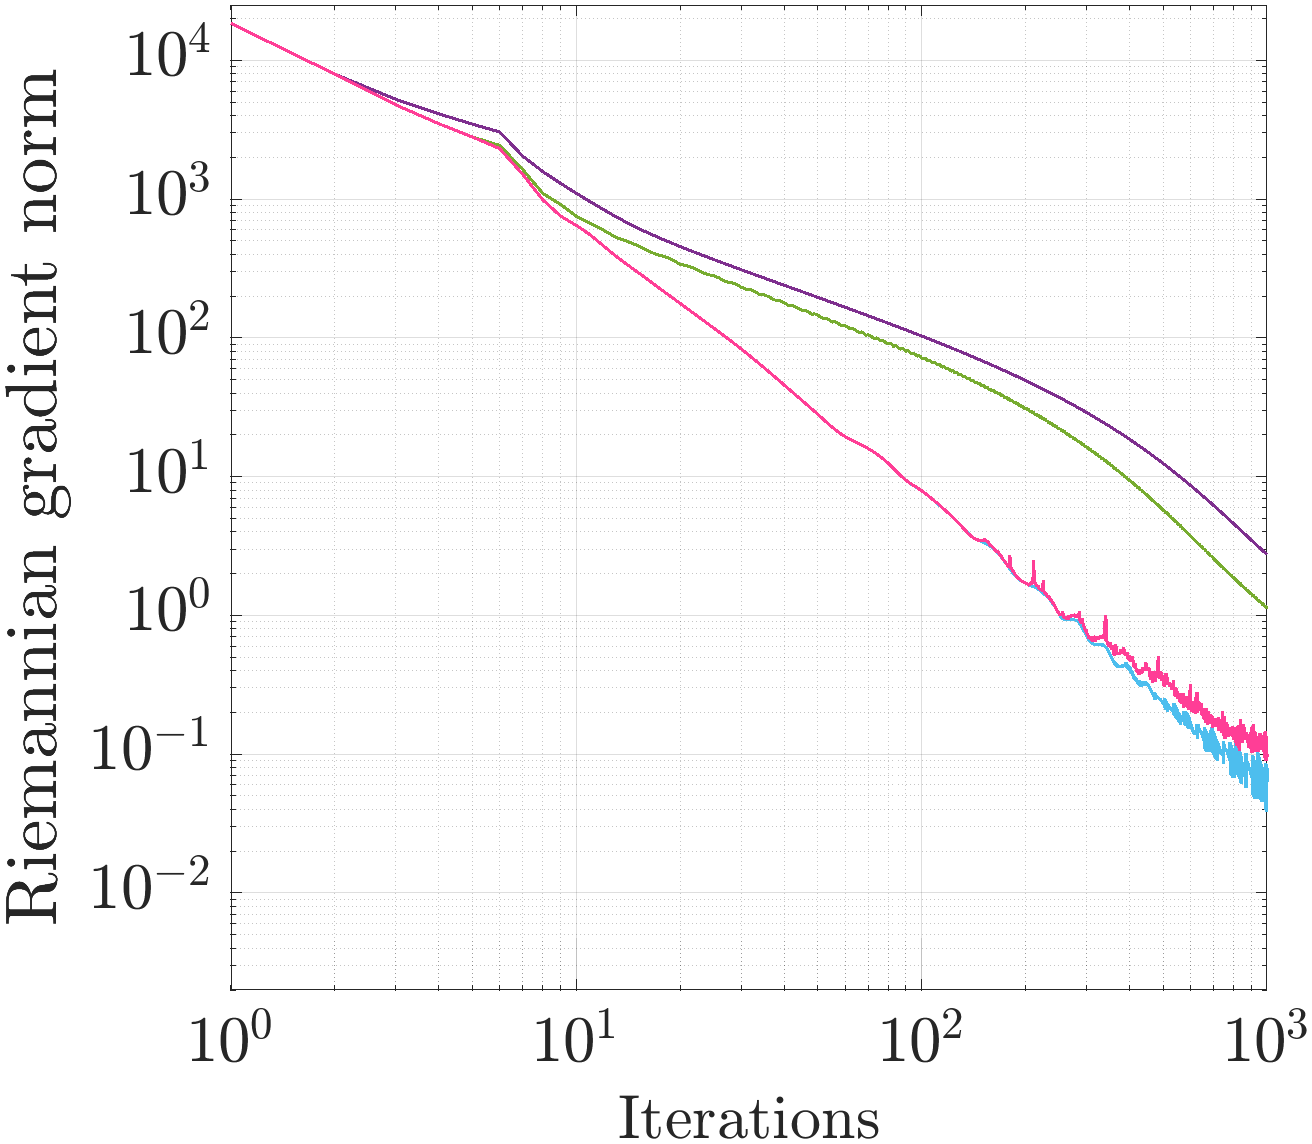
\includegraphics[trim =0mm 0mm 0mm 0mm,width=0.24\textwidth]{figures/cube_tests/rel_huber_g_50.png}}
	\end{tabular}
	\caption{The Riemannian gradient norms of the $\mm$, $\ammc$, $\ammd$ and $\amm$ \cite{fan2020mm} methods for distributed PGO with the \textbf{Huber loss kernel} on $5$, $10$ and $50$ robots. The results are averaged over $20$  Monte Carlo runs.}\label{fig::cube_g_huber} 
	\vspace{-0.5em}

	\begin{tabular}{cccc}
		\hspace{-0.5em}\subfloat[][$\ammd$ vs. $\mm$]{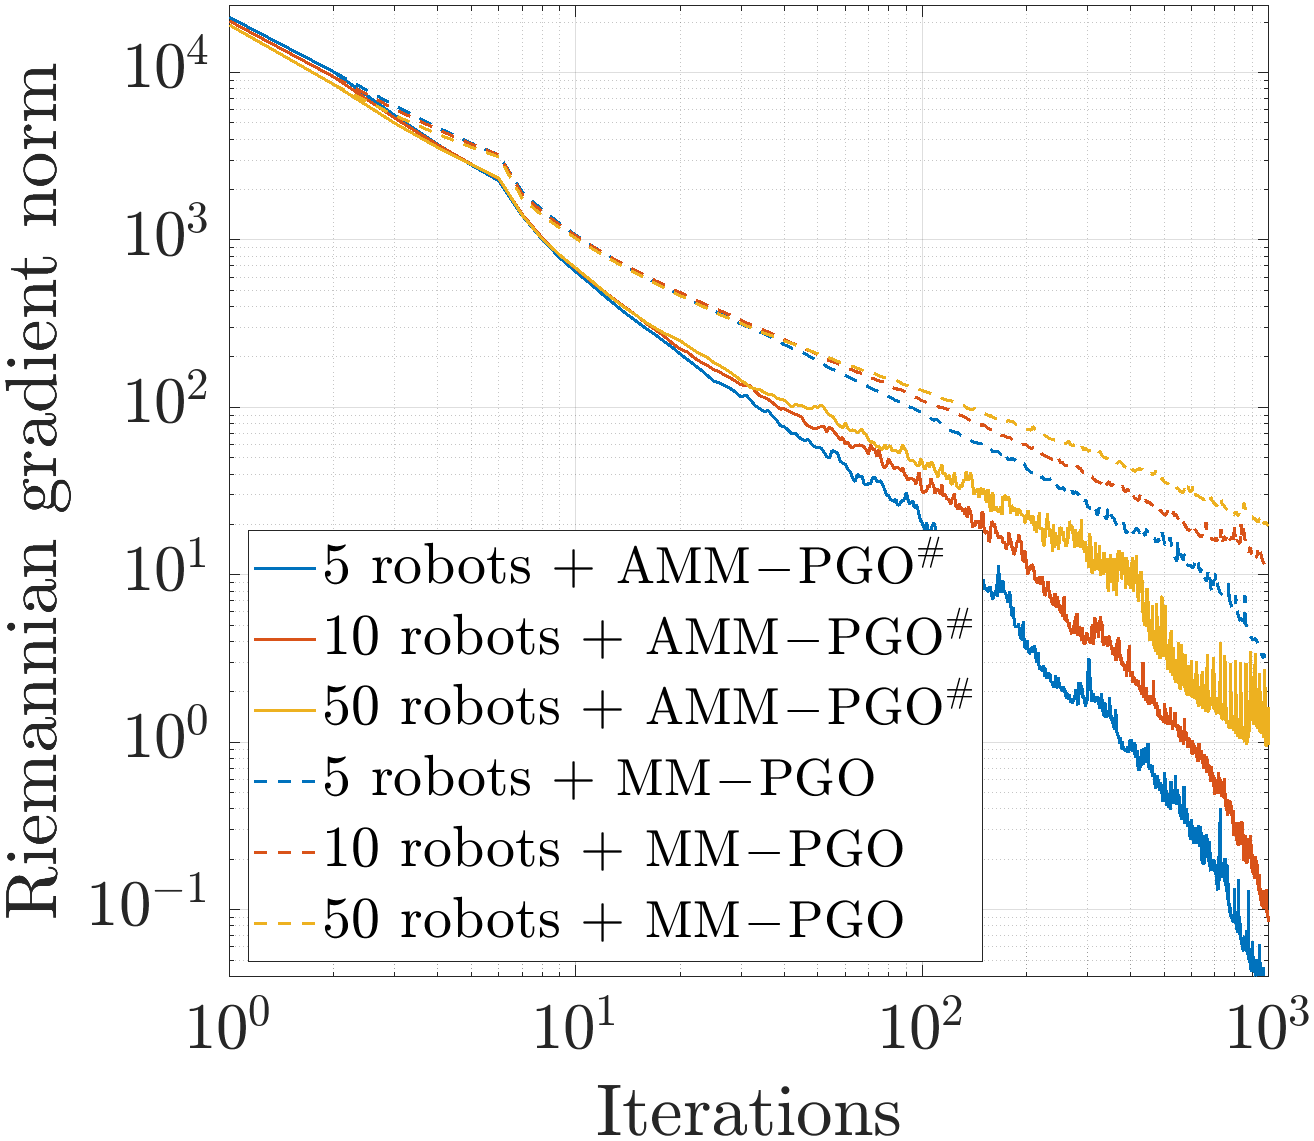
\includegraphics[trim =0mm 0mm 0mm 0mm,width=0.24\textwidth]{figures/cube_tests/rel_welsch_g.png}} &
		\hspace{-0.6em}\subfloat[][5 robots]{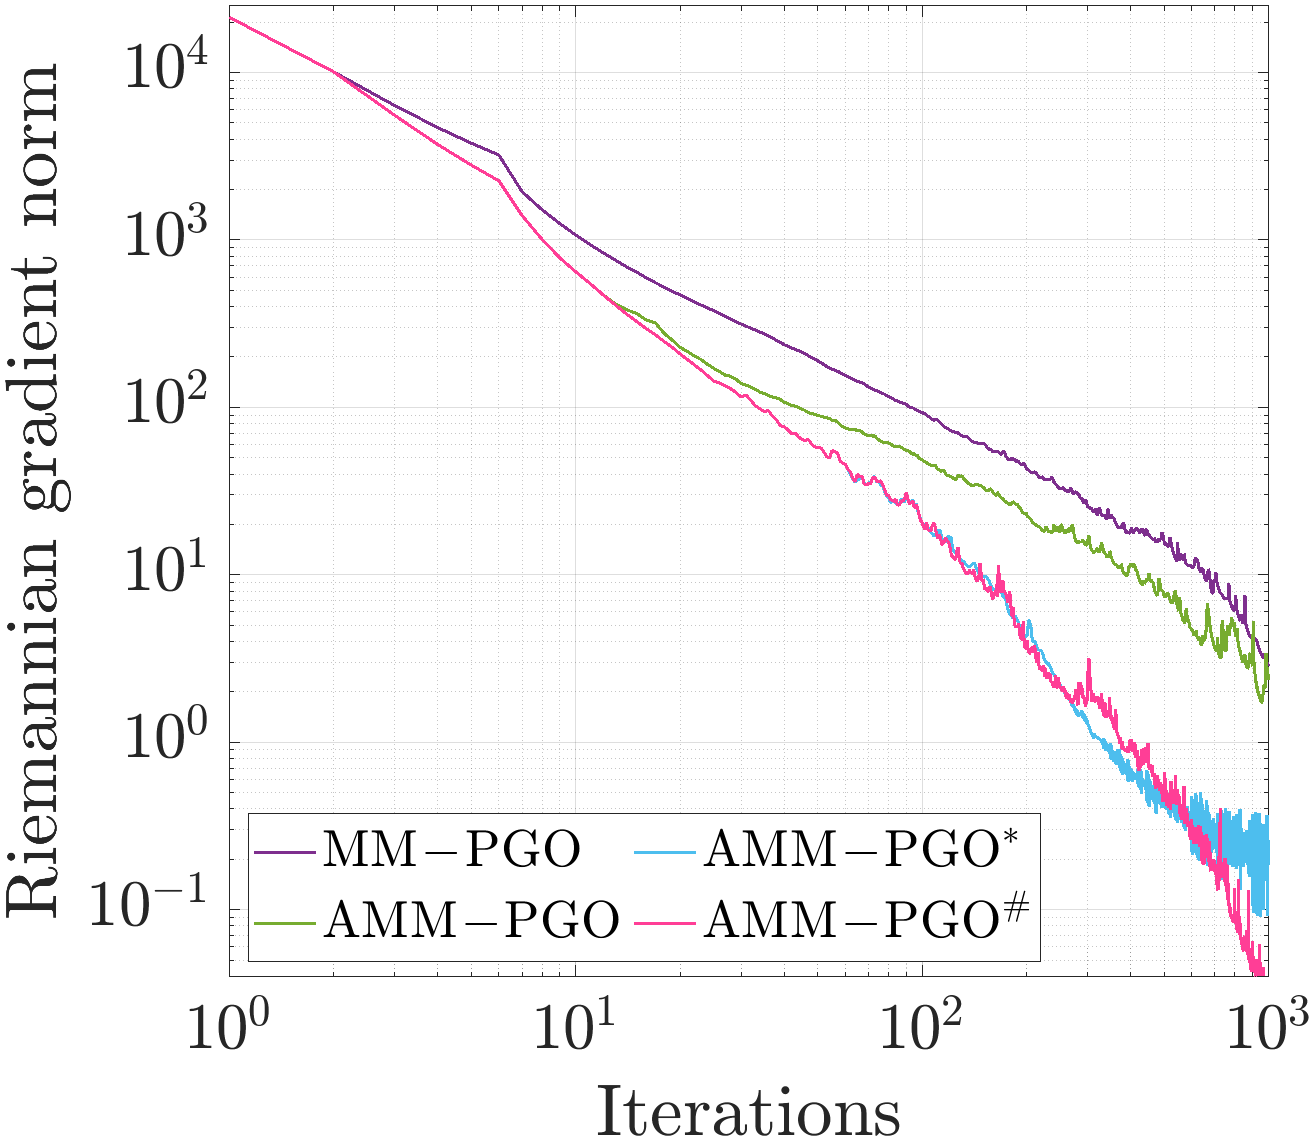
\includegraphics[trim =0mm 0mm 0mm 0mm,width=0.24\textwidth]{figures/cube_tests/rel_welsch_g_5.png}} &
		\hspace{-0.6em}\subfloat[][10 robots]{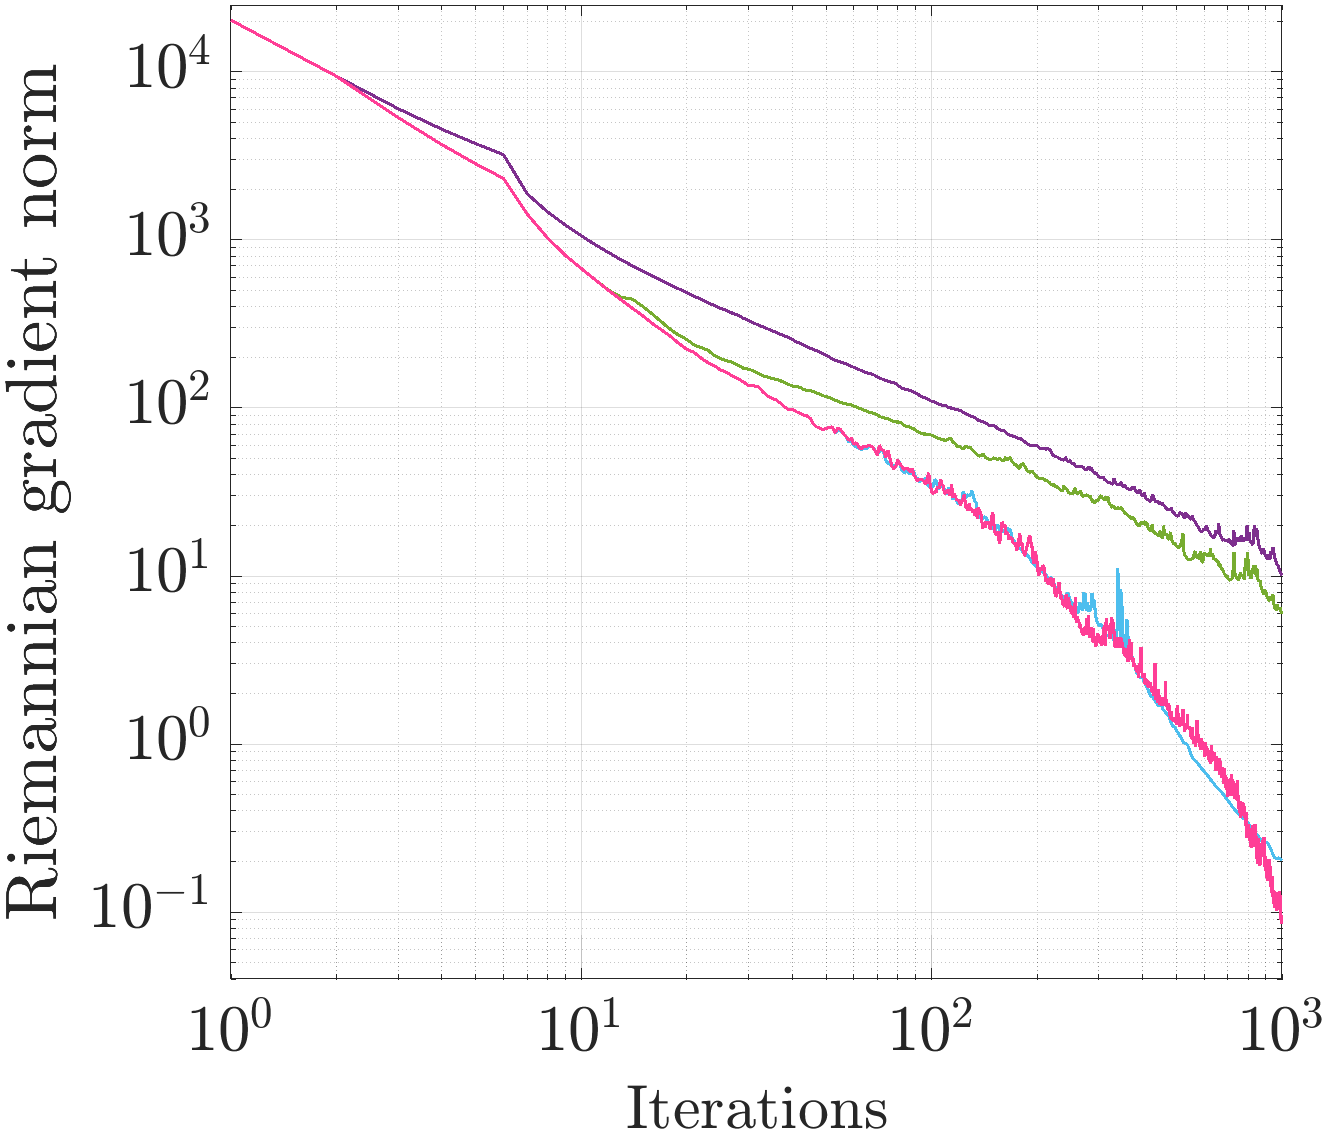
\includegraphics[trim =0mm 0mm 0mm 0mm,width=0.24\textwidth]{figures/cube_tests/rel_welsch_g_10.png}}&
		\hspace{-0.6em}\subfloat[][50 robots]{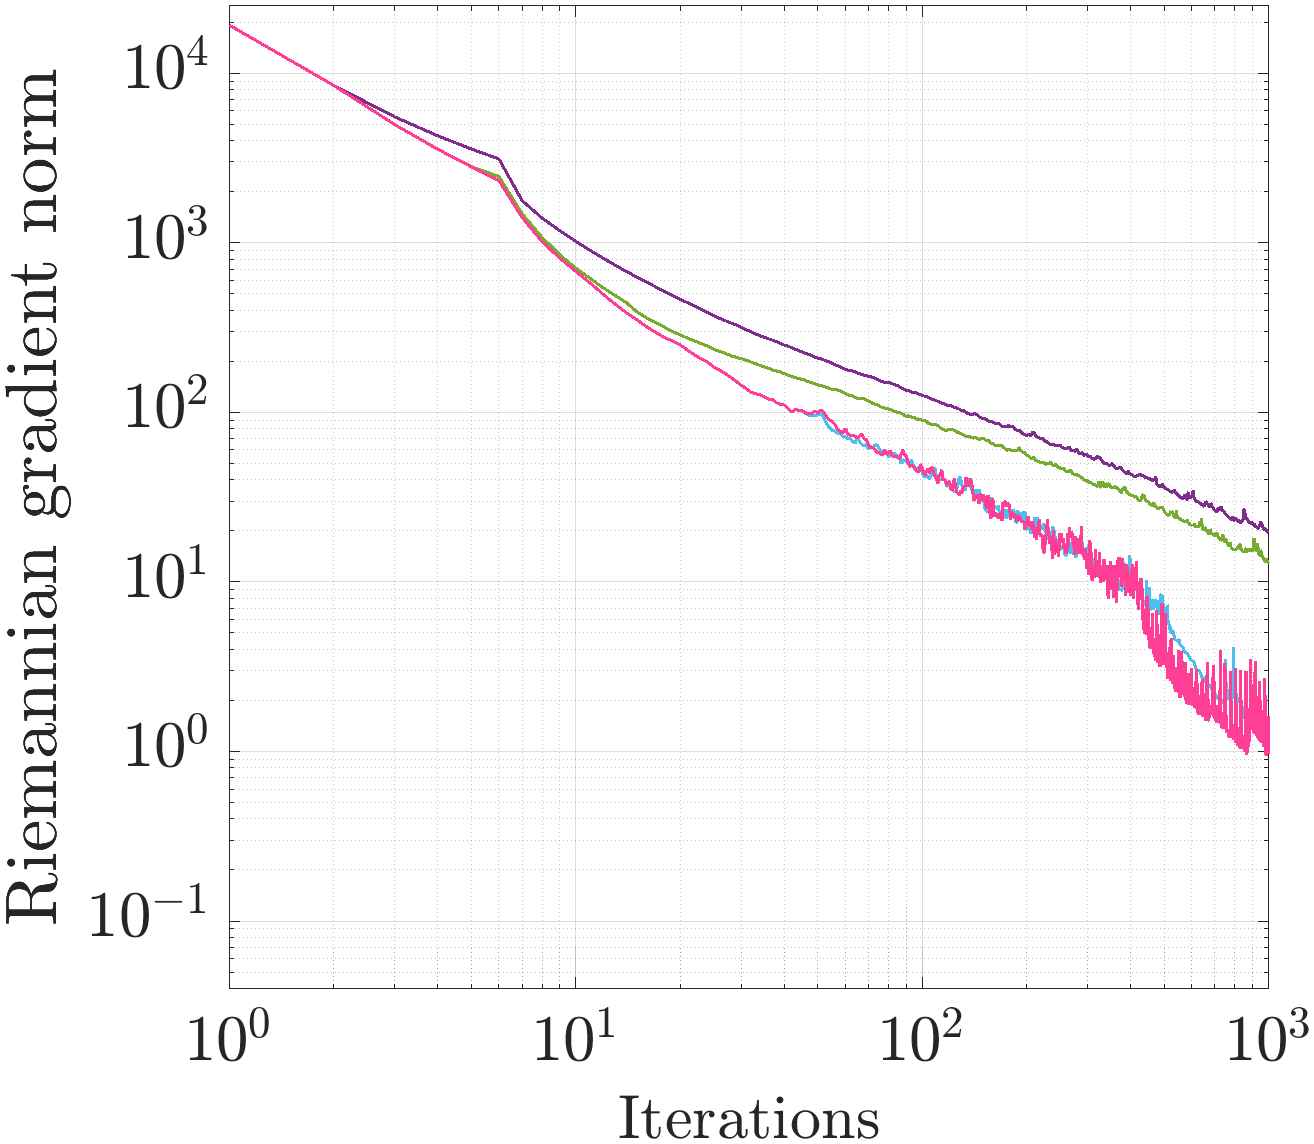
\includegraphics[trim =0mm 0mm 0mm 0mm,width=0.24\textwidth]{figures/cube_tests/rel_welsch_g_50.png}}
	\end{tabular}
	\caption{The Riemannian gradient norms of the $\mm$, $\ammc$, $\ammd$ and $\amm$ \cite{fan2020mm} methods for distributed PGO with the \textbf{Welsch loss kernel} on $5$, $10$ and $50$ robots. The results are averaged over $20$  Monte Carlo runs.}\label{fig::cube_g_gm}
	\vspace{-0.75em}
\end{figure*}
